\chapter{Aufgabe 1}

\noindent
Vor der semantischen Analyse beginnen wir zunächst mit einer Strukturanalyse: Welche Symbole kommen besonders häufig vor?\\
Wenn wir davon ausgehen, dass der Text in deutscher Sprache vorliegt, können wir bei ausreichender Länge des Textes hier eine erste Zuordnung vornehmen, und das am häufigsten vorkommende Symbol durch den in der deutschen Sprache am häufigsten vorkommenden Buchstaben ersetzen\footnote{
    wissenschaftl. Quellen hierzu bspw. \url{https://www.ids-mannheim.de/digspra/kl/projekte/methoden/derewo}, abgerufen 30.03.2025
}.
Hilfreich sind außerdem Statistiken über Anfangsbuchstabenhäufigkeit, mit deren Hilfe dann kürzere Symbolketten zu Artikeln, Subjunktionen und Adverbien (\textit{die}, \textit{wenn}, \textit{dann} usw.) aufgelöst werden können.\\
Die zur Lösung der Aufgabe verwendeten Buchstabenhäufigkeiten finden sich in den Tabellen~\ref{tab:bh_anfang} sowie~\ref{tab:bh_fliess}\footnote{
    \url{https://de.wikipedia.org/wiki/Buchstabenhäufigkeit}, abgerufen 30.03.2025
}.\\

\subsection*{Strukturanalyse}
\noindent
Eine Zählung der Symbole ergibt bspw., dass das \textbf{Sonnensymbol} besonders häufig vorkommt (21-mal), gefolgt von dem \textbf{Bombensymbol} (12-mal).\\

\noindent
Auffällig ist in dem Text die Symbolkette \textbf{DaumenRunter Wimpel}, die direkt nach einem Komma vorkommt - hier handelt es sich also um ein Wort bestehend aus zwei Buchstaben, von dem es im Deutschen - relativ gesehen - wenige gibt (\textit{im}, \textit{am}, \textit{an}, \textit{um}, \textit{ob}, \textit{so}, \ldots).\\

\noindent
Wir setzen an dieser Stelle den Hebel \textit{Buchstabenhäufigkeit} an, um eine erste Wahrscheinlichkeit (informell) zu ermitteln, ob \textbf{Wimpel} für ein \textbf{N} stehen könnte.
Da der Wimpel nur 3-mal im Text vorkommt, ein \textbf{N} entsprechend der Chiffratlänge aber häufiger vorkommen müsste (basierend auf der statistischen Häufigkeit in deutschen Fließtexten), schließen wir diese Möglichkeit zunächst aus.
Wir orientieren uns an Buchstaben, die weniger häufig vorkommen, wie \textbf{B}, \textbf{M}, \textbf{O}.\\

\noindent
Zunächst schließen wir einen Konsonanten an Stelle des \textbf{Wimpels} aus - \textbf{DaumenRunter} müsste dann ein Vokal sein, und wir haben den Fall, dass \textbf{DaumenRunter} in einer Symbolkette 2-mal hintereinander vorkommt, und zwar in Wort 13.
Das schauen wir uns genauer an.\\
Wir versuchen uns an \textbf{DaumenRunter Wimpel} mit \textbf{S O} und treffen an Wort 13 auf das \textbf{Sonnensymbol} und das \textbf{Schneeflockensymbol}, wobei das Schneeflockensymbol insgesamt 11-mal in dem Chiffrat vorkommt.

\subsection*{Semantische Analyse}
Ausgehend von der Häufigkeit der Buchstaben versuchen wir uns an einer \textbf{Known-Plaintext Attack} (vgl.~\cite[50]{ITS3}): Wir suchen ein Wort, das ein \textit{Doppel-S} enthält, als zweiten Buchstaben ein \textit{E}.
Der vorletzte Buchstabe - substituiert durch das \textbf{Bombensymbol} - kommt als zweithäufigster Buchstabe in dem Chiffrat vor.
Wir orientieren uns an der statistischen Buchstabenhäufigkeit und ersetzen durch \textit{N} (laut Tabelle~\ref{tab:bh_fliess}).\\

\noindent
Wir haben

\begin{equation}\notag
\texttt{\_ E \_ S \_ \_ \_ \_ E S S E \_ \_ N \_}
\end{equation}

\noindent
Durch den \textbf{fachlichen Bezug} des Themas kommen wir an der Stelle schnell auf das Wort

\begin{equation}\notag
\texttt{V E R S C H L U E S S E L U N G}
\end{equation}

\noindent
Damit stehen uns schon eine ganze Reihe von Buchstaben zur Verfügung.
Wir ersetzen entsprechend die Buchstaben in der Tabelle (siehe Abbildung~\ref{fig:decode}) und nutzen hierbei die Buchstabenhäufigkeiten sowie systematisches Ab- und Herleiten.\\
Wir lösen letztendlich auf zu\\

\noindent
\texttt{WIRD DER BEGRIFF KRYPTOGRAPHIE}\\
\texttt{VERWENDET, SO DENKT MAN ZUNÄCHST}\\
\texttt{AN PRAKTIKEN ZUR VERSCHLÜSSELUNG}\\
\texttt{VON DATEN, DIE AUCH ALS}\\
\texttt{GEHEIMSCHRIFT BEZEICHNET WERDEN}\\

\begin{figure}
    \centering
    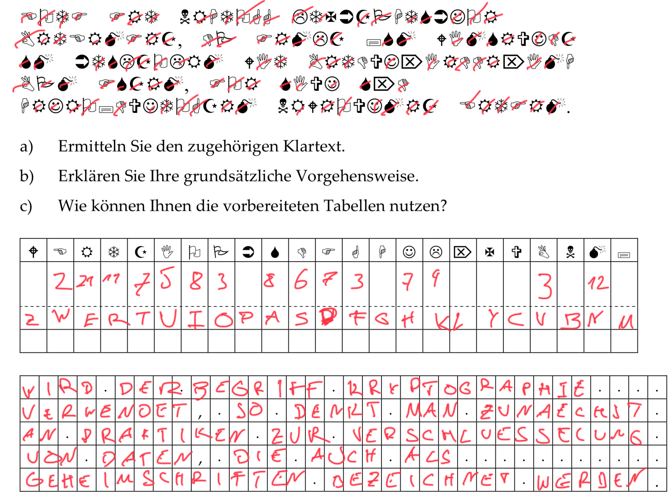
\includegraphics[scale=0.5]{aufgabe 1/img/decode}
    \caption{Verwendung der Symboltabelle und der Platzhalter zur Entschlüsselung des Chiffrats. (Quelle: eigener Screenshot)}
    \label{fig:decode}
\end{figure}




\begin{table}[h!]
    \setlength{\tabcolsep}{0.5em}
    \def\arraystretch{1.5}
    \centering
    \begin{tabular}{|c|c|l|}
        \hline
        \textbf{Platz} & \textbf{Buchstabe} & \textbf{Relative Häufigkeit} \\
        \hline
        1.  & E  & 17{,}40\,\% \\  \hline
        2.  & N  & 9{,}78\,\% \\ \hline
        3.  & I  & 7{,}55\,\% \\ \hline
        4.  & S  & 7{,}27\,\% \\ \hline
        5.  & R  & 7{,}00\,\% \\ \hline
        6.  & A  & 6{,}51\,\% \\ \hline
        7.  & T  & 6{,}15\,\% \\ \hline
        8.  & D  & 5{,}08\,\% \\ \hline
        9.  & H  & 4{,}76\,\% \\ \hline
        10. & U  & 4{,}35\,\% \\ \hline
        11. & L  & 3{,}44\,\% \\ \hline
        12. & C  & 3{,}06\,\% \\ \hline
        13. & G  & 3{,}01\,\% \\ \hline
        14. & M  & 2{,}53\,\% \\ \hline
        15. & O  & 2{,}51\,\% \\ \hline
        16. & B  & 1{,}89\,\% \\ \hline
        17. & W  & 1{,}89\,\% \\ \hline
        18. & F  & 1{,}66\,\% \\ \hline
        19. & K  & 1{,}21\,\% \\ \hline
        20. & Z  & 1{,}13\,\% \\ \hline
        21. & P  & 0{,}79\,\% \\ \hline
        22. & V  & 0{,}67\,\% \\ \hline
        23. & \ss{} & 0{,}31\,\% \\ \hline
        24. & J  & 0{,}27\,\% \\ \hline
        25. & Y  & 0{,}04\,\% \\ \hline
        26. & X  & 0{,}03\,\% \\ \hline
        27. & Q  & 0{,}02\,\% \\ \hline
    \end{tabular}
    \caption{Häufigkeit von Buchstaben in Fließtexten dt. Sprache. (Quelle: Wikipedia)}
    \label{tab:bh_fliess}
\end{table}


\begin{table}[h!]
    \setlength{\tabcolsep}{0.5em}
    \def\arraystretch{1.5}
    \centering
    \begin{tabular}{|c|c|l|}
        \hline
        \textbf{Platz} & \textbf{Buchstabe} & \textbf{Relative Häufigkeit} \\
        \hline
        1. & D & 14{,}2\,\% \\ \hline
        2. & S & 10{,}8\,\% \\ \hline
        3. & E & 7{,}8\,\% \\ \hline
        4. & I & 7{,}1\,\% \\ \hline
        5. & W & 6{,}8\,\% \\ \hline
    \end{tabular}
    \caption{Häufigkeit von Anfangsbuchstaben in Fließtexten dt. Sprache. (Quelle: Wikipedia)}
    \label{tab:bh_anfang}
\end{table}